
\section{Introduction to Resource Sharing in Real-Time Systems}
A new process in real-time system starts with assigning different resources. These resources may vary from data structures, variables, memory (both volatile and non-volatile), files, registers, I/O to processors and others- depending on the task. As stated by~\cite{JiacunWang.2017}, “Starting a new process is a heavy job for the OS, which includes allocating memory, creating data structures, and coping code.” In real-time systems, the process of resource sharing is crucial for ensuring that tasks can execute without unnecessary delays or conflicts and thus meeting their deadlines. As stated by~\cite{JiacunWang.2017} also, "Real-time embedded systems are often run in highly resource-constrained environments, which make the system design and performance optimization quite challenging."- thus implying the importance of sharing resources. The process needs to follow certain protocols. These protocols can be defined as "a set of rules that govern when and under what conditions each request for resource is granted and how tasks requiring resources are scheduled."~\cite{JiacunWang.2017}. Whereas it is also mentioned by~\cite{dosSantos.2023} that, "Any concurrent operating system (OS)must offer protocols to control the access to resources shared (i.e., a piece of code, such as data structures, I/O devices, buffers, and so on) by competing tasks, thus ensuring mutual exclusion in their respective critical sections (a code segment where shared variables can be accessed)". To further emphasize the importance, a well-designed access control protocol is critical for preventing deadlocks from occurring~\cite{JiacunWang.2017}. Although, there is no protocol that can eliminate priority inversion, the goal of access control is to keep the blocking time of the higher priority tasks under control~\cite{JiacunWang.2017}.\\  

For better understanding of how these protocols manage resources allocation among different tasks, a situation can be considered where 3 tasks (J1, J2 and J3) are running in a real-time system. There, are m type of resources in a system, namely R1, R2, R3………, Rm where each resource comprises $\eta_i$ number of indistinguishable units of Ri, i=1, 2, …., m. When a task requests $\rho_i$ units of a resource Ri, request is sent to kernel to lock them and can be denoted as L(Ri, $\rho_i$). When the resource is longer needed by the task, it is unlocked and can be denoted by U(Ri, $\rho_i$). As plentiful resources have no effect on scheduling plentiful resources have no effect on scheduling~\cite{UniversityofGlasgow}, we can avoid considering them here. Also to be considered here- only the serially reusable resources, which are "one that can be used safely by one task at a time and is not depleted by that use"~\cite{JiacunWang.2017}. The examples of these resources are devices, files, databases, and semaphores~\cite{JiacunWang.2017}. The access to resources by every task will be controlled by locking mechanisms.
% ...existing code...

\begin{figure}[H]
    \centering
    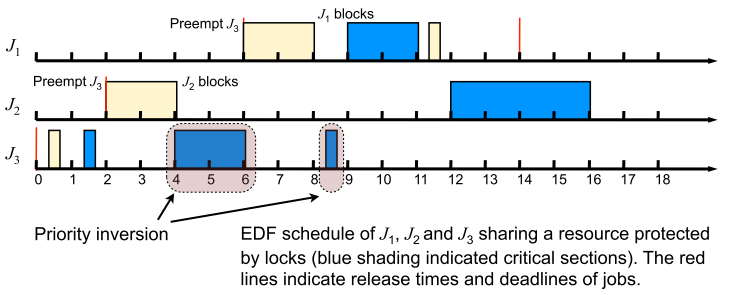
\includegraphics[width=0.7\textwidth]{Figures/EDF_scheduling_of_tasks_while_resources_are_protectd_by_locks.png}
    \caption{EDF scheduling of tasks while resources are protected by locks~\cite{UniversityofGlasgow.}}
    \label{fig:EDF_scheduling_of_tasks_while_resources_are_protected_by_locks}
\end{figure}

% ...existing code...